\cleardoublepage
\chapter{Neurophysiological and behavioral factors associated with a high DRF}
\label{disc:drf}

\section{Summary of the results}
\label{disc:drf:summary}

One of the major objectives of the present thesis was to investigate the neurophysiological and behavioral correlates of inter-individual variability in dream recall frequency (DRF). Based on previous findings, we hypothesized that DRF is associated with a specific brain functioning during both sleep and wakefulness. To test this hypothesis, we compared the brain activity, sleep parameters, cognitive performances and personality traits of individuals who recall dreams almost every day (high dream recallers, HR) and individuals who hardly ever recall one (low dream recallers, LR). The main findings are summarized in Fig \ref{fig:disc:drf:summary}.

In the first study (see section \ref{res:arousal}), we performed an in-depth investigation of the sleep macro and micro-structure of HR and LR by re-analyzing the polysomnographic recordings of  \citet{eichenlaub_brain_2014}. The analysis included arousals (i.e. short awakenings lasting at least 3 sec, and scored independently of the sleep stages), spindles, K-complexes, rapid eye movements and muscle twitches. We did not find any significant between-group differences for any of these parameters. Our interpretation of these findings is that, most probably, sleep microstructural features are not crucial factors to explain DRF variability.

By contrast, we observed that full awakenings (i.e > 15 seconds) were longer, whatever the sleep stages, in HR than in LR (roughly 2 vs 1 min respectively). While the total duration of intra-sleep wakefulness was higher in HR than in LR, it should be noted that the number of intra-sleep awakenings was not different between the two groups. Thus, it appears that the duration of intra-sleep wakefulness during sleep seems to be the best predictor of inter-individual differences in DRF. This result provides yet another evidence in favor of the so-called arousal-retrieval model (see section \ref{sec:dream-recall:theories:arousal}, \citealp{koulack_dream_1976}), which states that a short period of wakefulness must occur immediately after dreaming in order to transfer the dream content from short-term memory to long term memory. Our findings constitute an essential contribution to this model by showing that awakenings must be of sufficient duration to allow successful encoding of dreams into memory. We proposed, in accordance with previous findings \citep{campbell_perception_1981}, that an awakening should last at minimum two minutes to allow for successful memory encoding.

On this point, it should be noted that the author of this thesis contributed to a study aiming at investigating, by means of human intra-cortical EEG, the temporal dynamic of reactivation of brain regions involved in memory processing during arousals (ranging from 3 sec to 2 minutes). Preliminary results (not reported here) showed that the spectral composition of hippocampal EEG signal during these arousals was intermediate between that of sleep and wakefulness activities, and that this activation was modulated by the awakening duration. Furthermore, we showed that hippocampus activity during these arousals was different during NREM and REM sleep, thus providing some evidences about a functional dichotomy between these two sleep stages regarding memorization processes, that could in turn explain the well-known higher dream recall rate following awakening from REM sleep than NREM sleep \citep{nielsen_review_2000}.

The visual scoring of arousals allowed us to address another issue, which is related to the finding of differential brain reactivity to auditory stimuli in high and low dream recallers (see section \ref{sec:dream-recall:param:neuro}). \citet{eichenlaub_brain_2014} has suggested that there might be a causal link between between neurophysiological responses to auditory stimuli (which are larger in HR) and intra-sleep wakefulness during sleep (which is greater in HR). In other words, the amplitude of brain responses to auditory stimuli could be predictive of subsequent awakening or arousal reactions, an observation that has been previously reported for nociceptive stimuli \citet{bastuji_laser_2008}. To test this hypothesis, we computed the auditory evoked potentials to arousing stimuli (i.e. inducing either an arousal or awakening) or non-arousing stimuli (i.e. stimuli that do not induce a disruption of the PSG signal). This comparison was not possible without the tedious and time-consuming visual scoring of arousals given that arousals are far more frequent than awakenings in a normal night of sleep, and are therefore needed to compute reliable and statistically valid evoked potentials.

Consistent with our hypothesis, we have shown that brain responses to auditory stimuli, in N2 sleep, were larger when followed by a subsequent arousing reaction. Importantly, this increase in the amplitude of the brain responses seemed to be stimulus-specific given that the amplitude was larger when arousing reactions were within 5 seconds after the stimulus compared to when they were between 5 and 15 seconds. Behaviorally, HR elicited a significantly greater proportion of stimuli followed by an arousing reaction than LR. Although it was not possible to compute between-group comparisons of the evoked potentials (because of a too few number of subjects in each group with sufficient arousing stimuli), these findings are significant because they provide the missing link between the greater brain reactivity observed in HR and the increased intra-sleep wakefulness during sleep.

\begin{figure}[!htbp]
	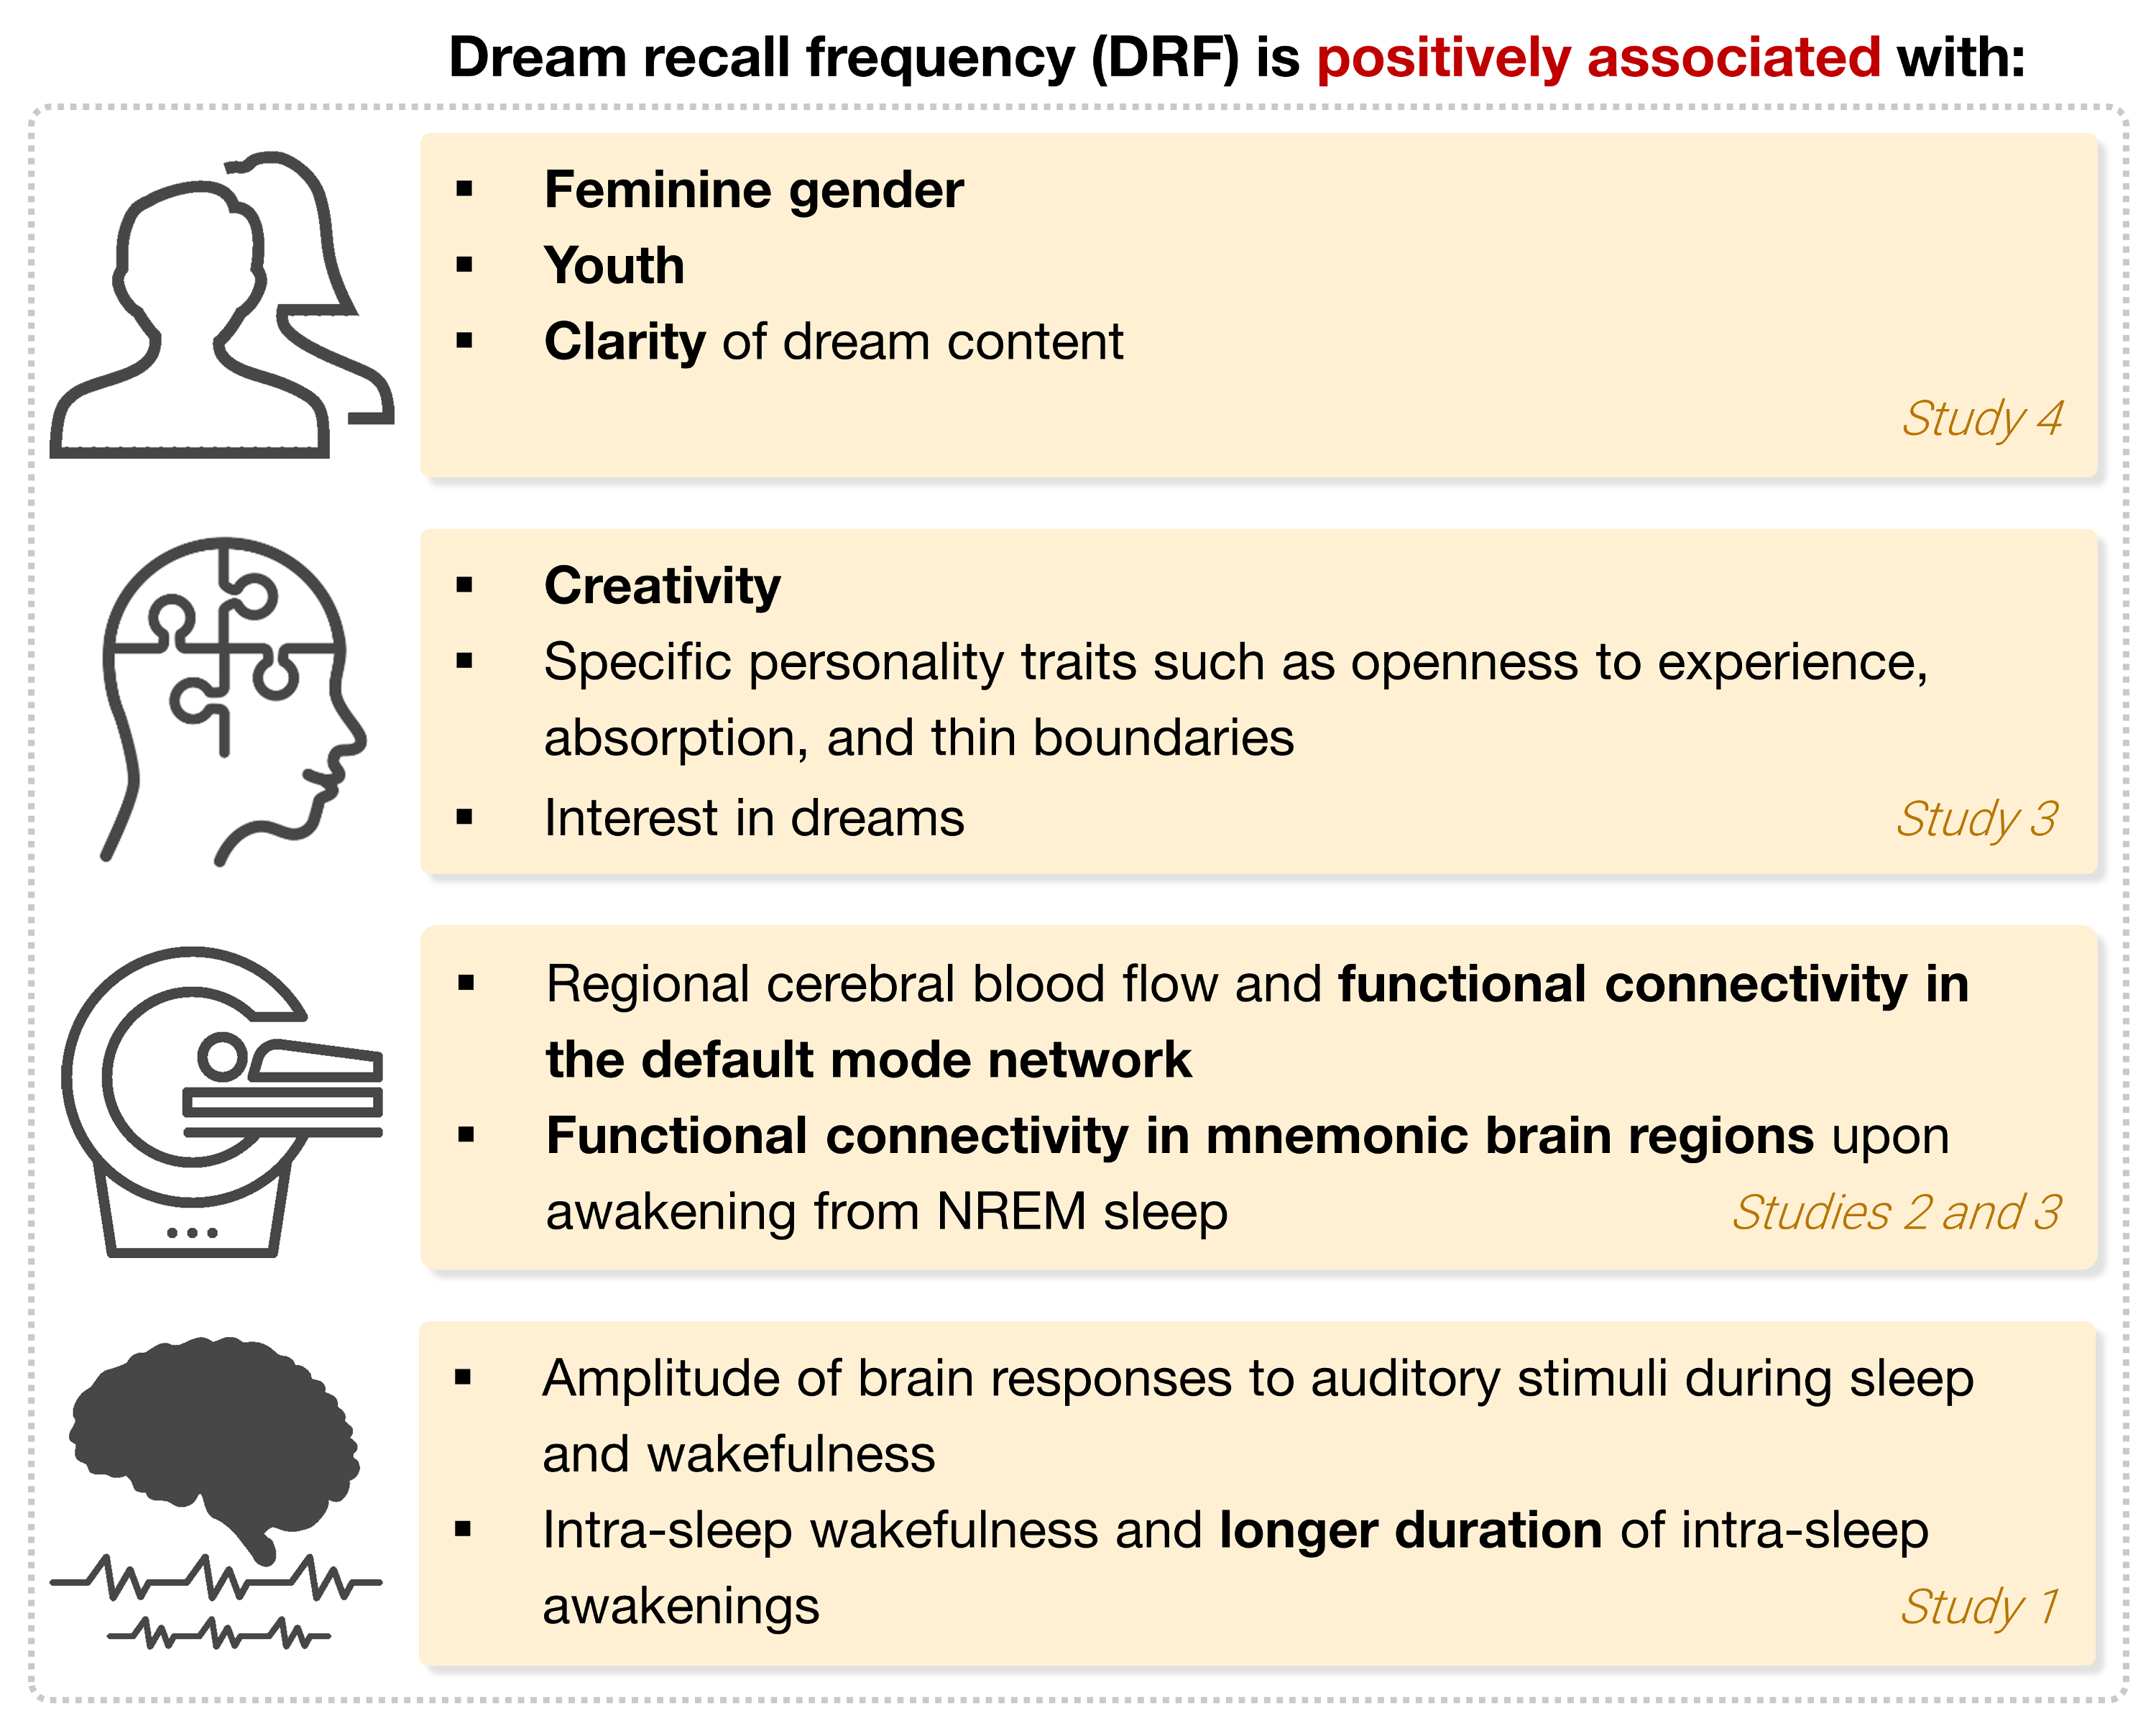
\includegraphics[width=\textwidth]{Fig/Discussion/HR_recap.png}
	\caption[Summary of the results on DRF]{Summary of the behavioral and neurophysiological differences observed between high and low dream recallers.}
	\label{fig:disc:drf:summary}
\end{figure}

\FloatBarrier

\section{A model of dream recall}
\label{disc:drf:model}

The results of the current thesis as well as those from previous works led us to propose a comprehensive and unified theory of dream recall, depicted in Fig \ref{fig:disc:drf:model}. The main assumption of this model is that dream recall hinges on the successful encoding of the dream short-term memory into a more stable long-term memory, which is only possible upon awakening from sleep.

The period following awakening from sleep is therefore critical in the successful encoding of the dream memory trace. This period is influenced on one side by state-factors such as the severity of sleep inertia, which is related to the physiological context (e.g. prior sleep stage and duration), and on the other side by traits factors such as the interest in dreams, which would result in a stronger focus on dream content immediately upon awakening and therefore less interferences within the encoding process. In more simple terms, it might be that individuals with a positive attitude toward their dreams may recall them better trough a voluntarily memory effort, while individuals with little or no interest towards their dreams may not do any effort to grasp the ephemeral dream memory. However this factor does not explain the full inter-individual variability in DRF given that even when awakened and asked to recall their dreams in controlled laboratory conditions, LR still reports less dream than HR \citep{eichenlaub_brain_2014, eichenlaub_resting_2014}.

Another crucial factor of this model in the process of dream recall relates to the salience of the dream content, i.e. the more salient a dream is (e.g. a vivid, bizarre, and highly emotional dream), the more likely it will be recalled. This idea was first proposed by \citet{cohen_test_1974} and received further support from studies showing that bizarreness  and emotionality enhance dream recall \citep{cipolli_bizarreness_1993, schredl_emotions_1998}.

%%%%%% SEE BLAGROVE PACE SCHOTT 2010

\begin{figure}[!htbp]
	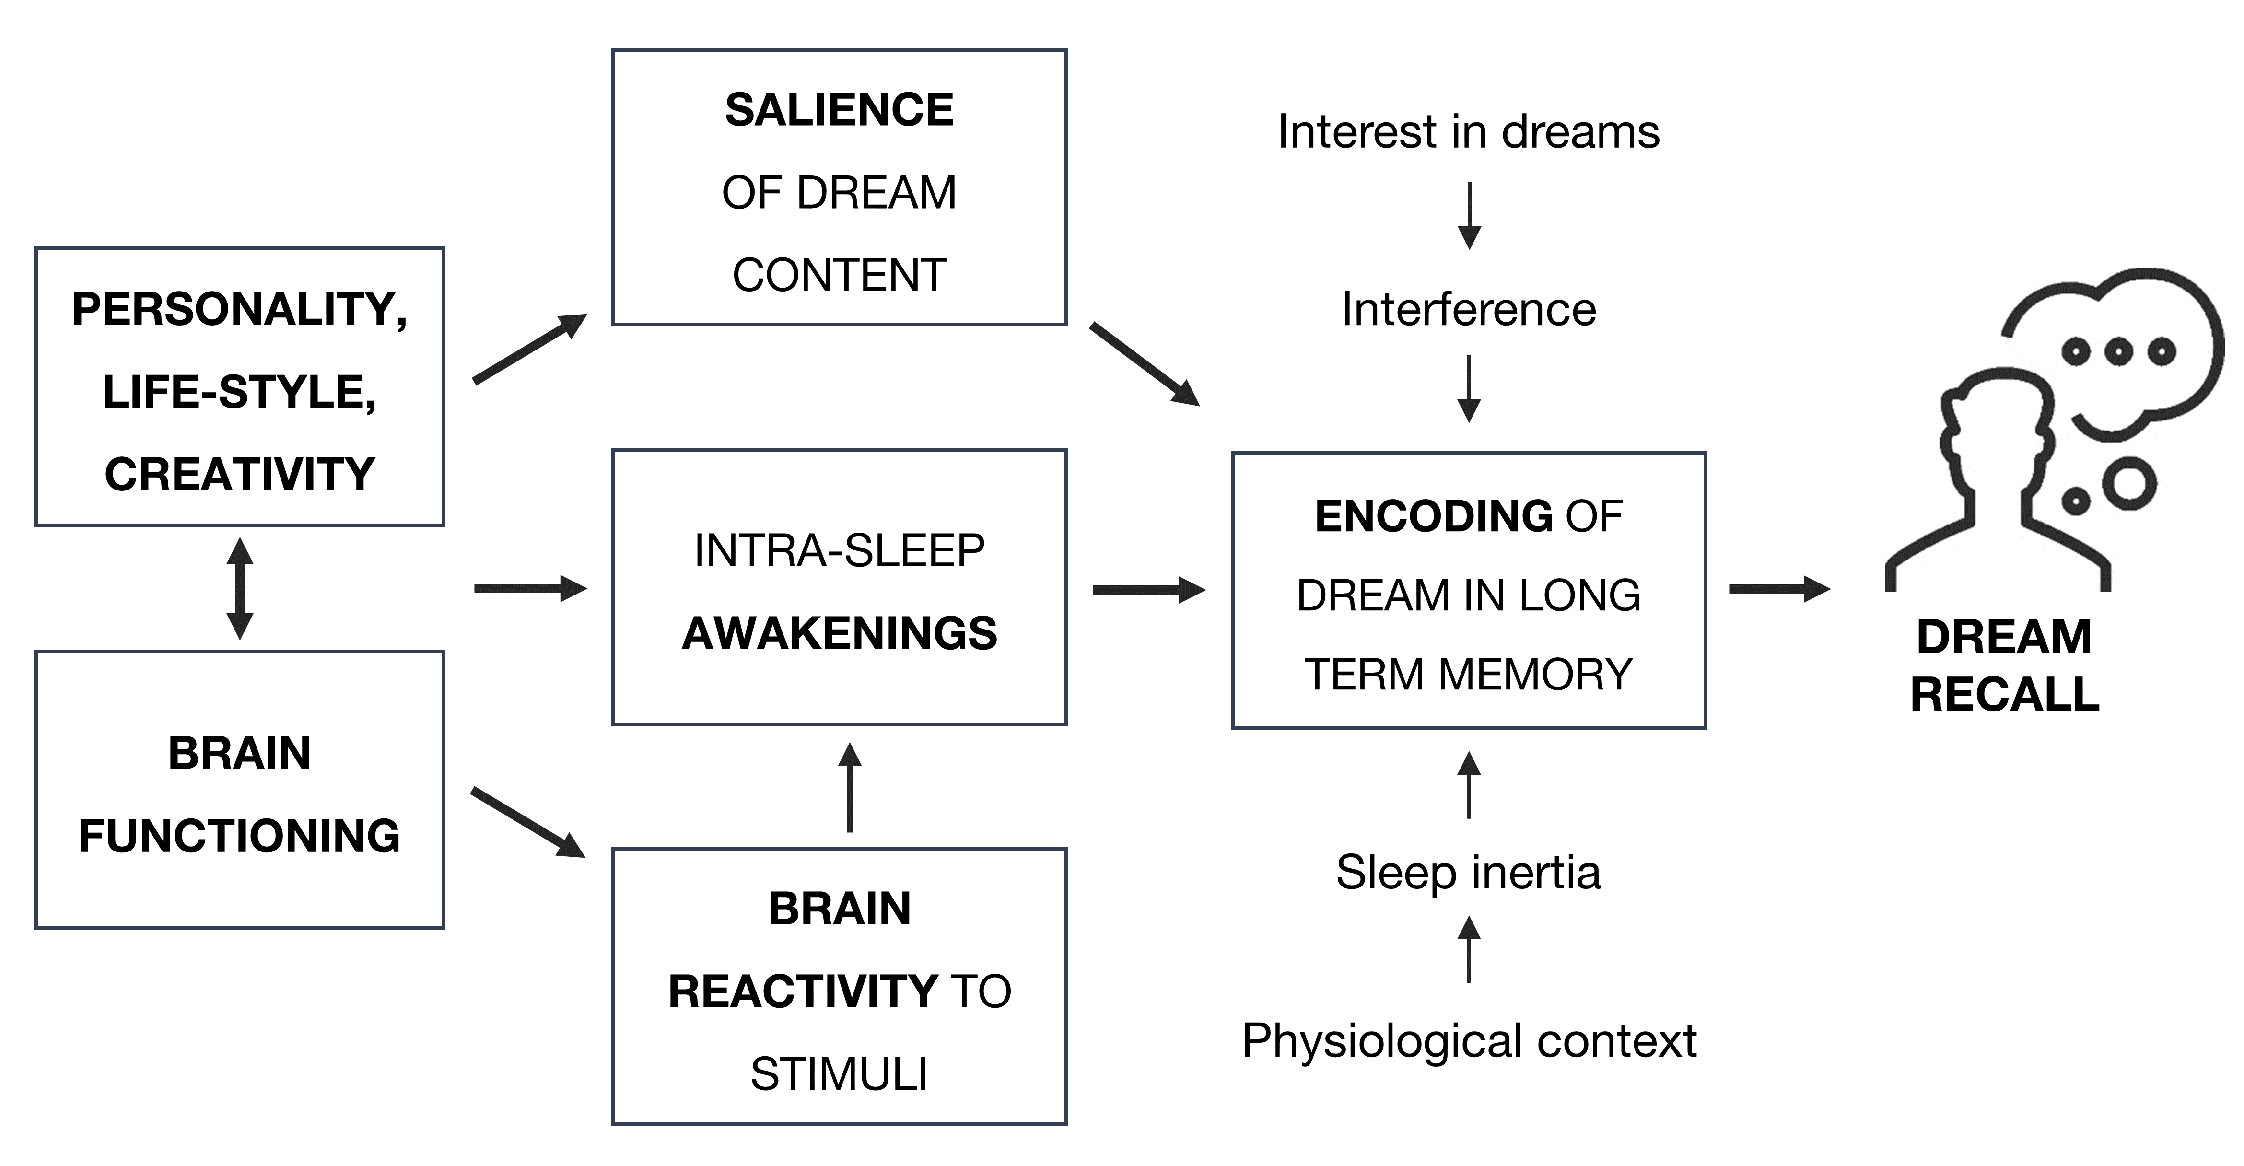
\includegraphics[width=\textwidth]{Fig/Discussion/schema_dream_recall.png}
	\caption[A comprehensive and unified model of dream recall]{A comprehensive and unified model of dream recall.}
	\label{fig:disc:drf:model}
\end{figure}

\section{Perspectives}
\label{disc:drf:perspectives}


%%%%%%%%%%%%%%%%%%%%%%%%%%%%%%%%%%%%%%%%%%%%%%%%%%%%%%%%%%%%%%%%%%%%%%%%%%%%%%%
\cleardoublepage
\chapter{The relationship between waking life and dream content}
\label{disc:wle}

%%%%%%%%%%%%%%%%%%%%%%%%%%%%%%%%%%%%%%%%%%%%%%%%%%%%%%%%%%%%%%%%%%%%%%%%%%%%%%%
\cleardoublepage
\chapter{Methodological development}
\label{disc:methods}

\section{A state-of-the-art open-source software}
\label{disc:methods:software}

SLEEP is a free, cross-platform and open-source graphical user interface dedicated to sleep reading, scoring and analysis. Initially designed for a personal use, it soon extended into a fully developed module with a comprehensive and intuitive interface. SLEEP has many advantages over other existing solutions. First, and perhaps most importantly, it is free and open-source. Second, it leverages the graphics processing unit to deliver cutting edge graphical performances. Third, it natively supports several commercial and public data file formats, thus making it accessible to the greatest possible number of people. Fourth, it implements several signal processing tools, as well as several automatic detections of sleep microstructural features. Fifth, it comes with an extensive documentation, a chat room and a peer-reviewed publication. In view of all these functionalities, one can reasonably conclude that SLEEP represents a state-of-the-art software in sleep research which should consequently benefit many. Furthermore, as the development of the software is still ongoing, novel functionalities will continue to be added. Some of these future perspectives are detailed in the section below.

\section{Future directions}
\label{disc:methods:future}

SLEEP includes so far 6 algorithms for detecting some of the most prominent features of each sleep stage, namely spindles, K-complexes, slow waves, rapid eye movements and muscle twitches. Two of these detections (i.e. spindles and K-complexes) were compared against a visual scoring reference and showed overall good performances. Yet, there are still opportunities for further enhancements and the detection algorithms were improved since the initial, published, version. An example of the updated spindles detection can be found in Fig \ref{fig:disc:methods:future:spindles}.

\begin{figure}[htb]
	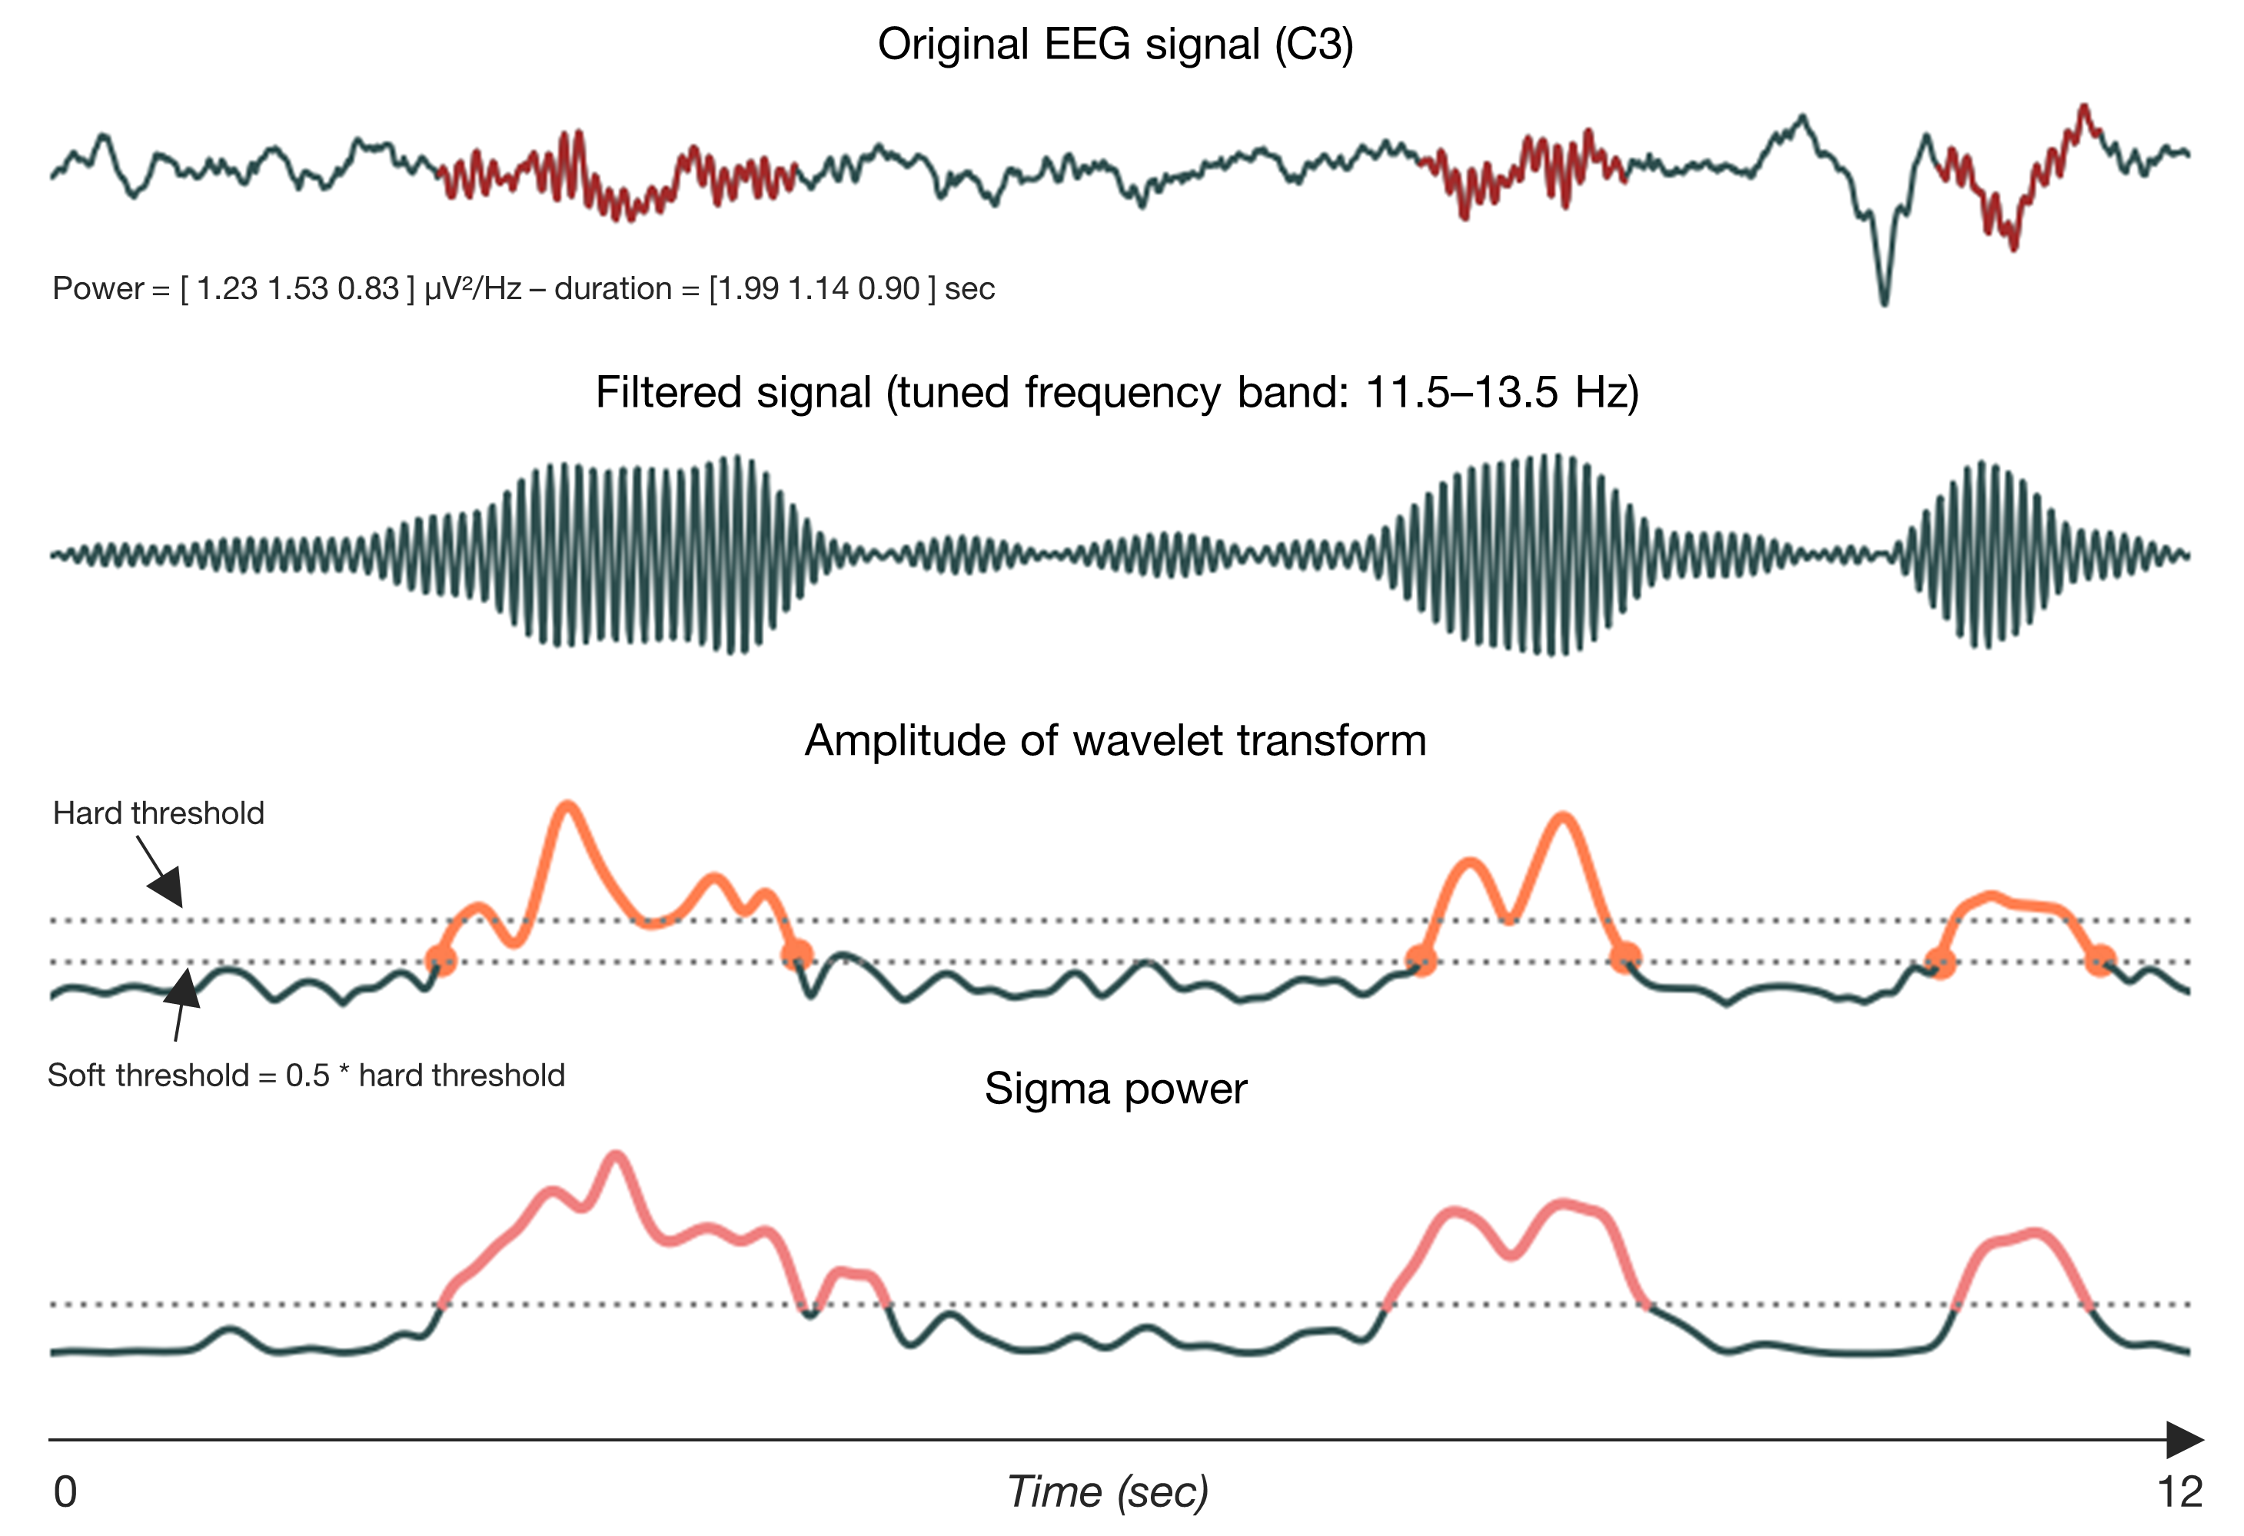
\includegraphics[width=\textwidth]{Fig/Discussion/spindles.png}
	\caption[Improved spindles detection algorithm]{\textbf{Improved spindles detection algorithm.} Compared to the initial algorithm (presented in chapter \ref{res:software}), the new spindles detection has several improvements. First, we implemented a data-driven tuning of the spindle frequency band by finding the peak spectral power within the sigma range. This step, described by \citet{berthomier_automatic_2007}, allows to accommodate for inter-individual variability of EEG signals, and is particularly useful when analyzing patients who tend to exhibit higher variability. Second, we now use both a hard and a soft threshold on the amplitude of the wavelet transform to determine more precisely the beginning and the end of each spindle. Finally, to allow users to better understand how the detection algorithm works, we implemented a function to plot the current figure for each desired time window.}
	\label{fig:disc:methods:future:spindles}
\end{figure}

Perhaps one of the most challenging issue in sleep research is the scoring of sleep stages. Currently, the gold standard remains visual scoring by an expert, which is time-consuming and subject to high inter-rater variability. There is therefore a crucial need for reliable and time-efficient algorithms capable of detecting sleep stages in healthy and patients alike. While recent years have witnessed a surge in automatic sleep scoring methods (e.g. \citealp{berthomier_automatic_2007, lajnef_learning_2015}), there is always a room for improvement and one of the ultimate goal of SLEEP software would therefore be to embed within the graphical user interface a function to perform automatic sleep scoring.

With this in mind, we are currently working on two distinct automatic sleep scoring methods, based on spectral feature extraction / microstructural detection (Fig \ref{fig:disc:methods:future:autoscore}), and on machine-learning algorithms, respectively. Preliminary results based on the former method show a 81\% agreement with a manually scored standard reference, a figure comprised within the range of human inter-scorer agreements (generally between 80 and 90\%, see \citealp{silber_visual_2007}). A similar agreement was obtained using the second, machine-learning based automatic sleep scoring method. Future developments will be needed to get the most out of these two methods to provide a state-of-the-art algorithm.

\begin{figure}[htb]
	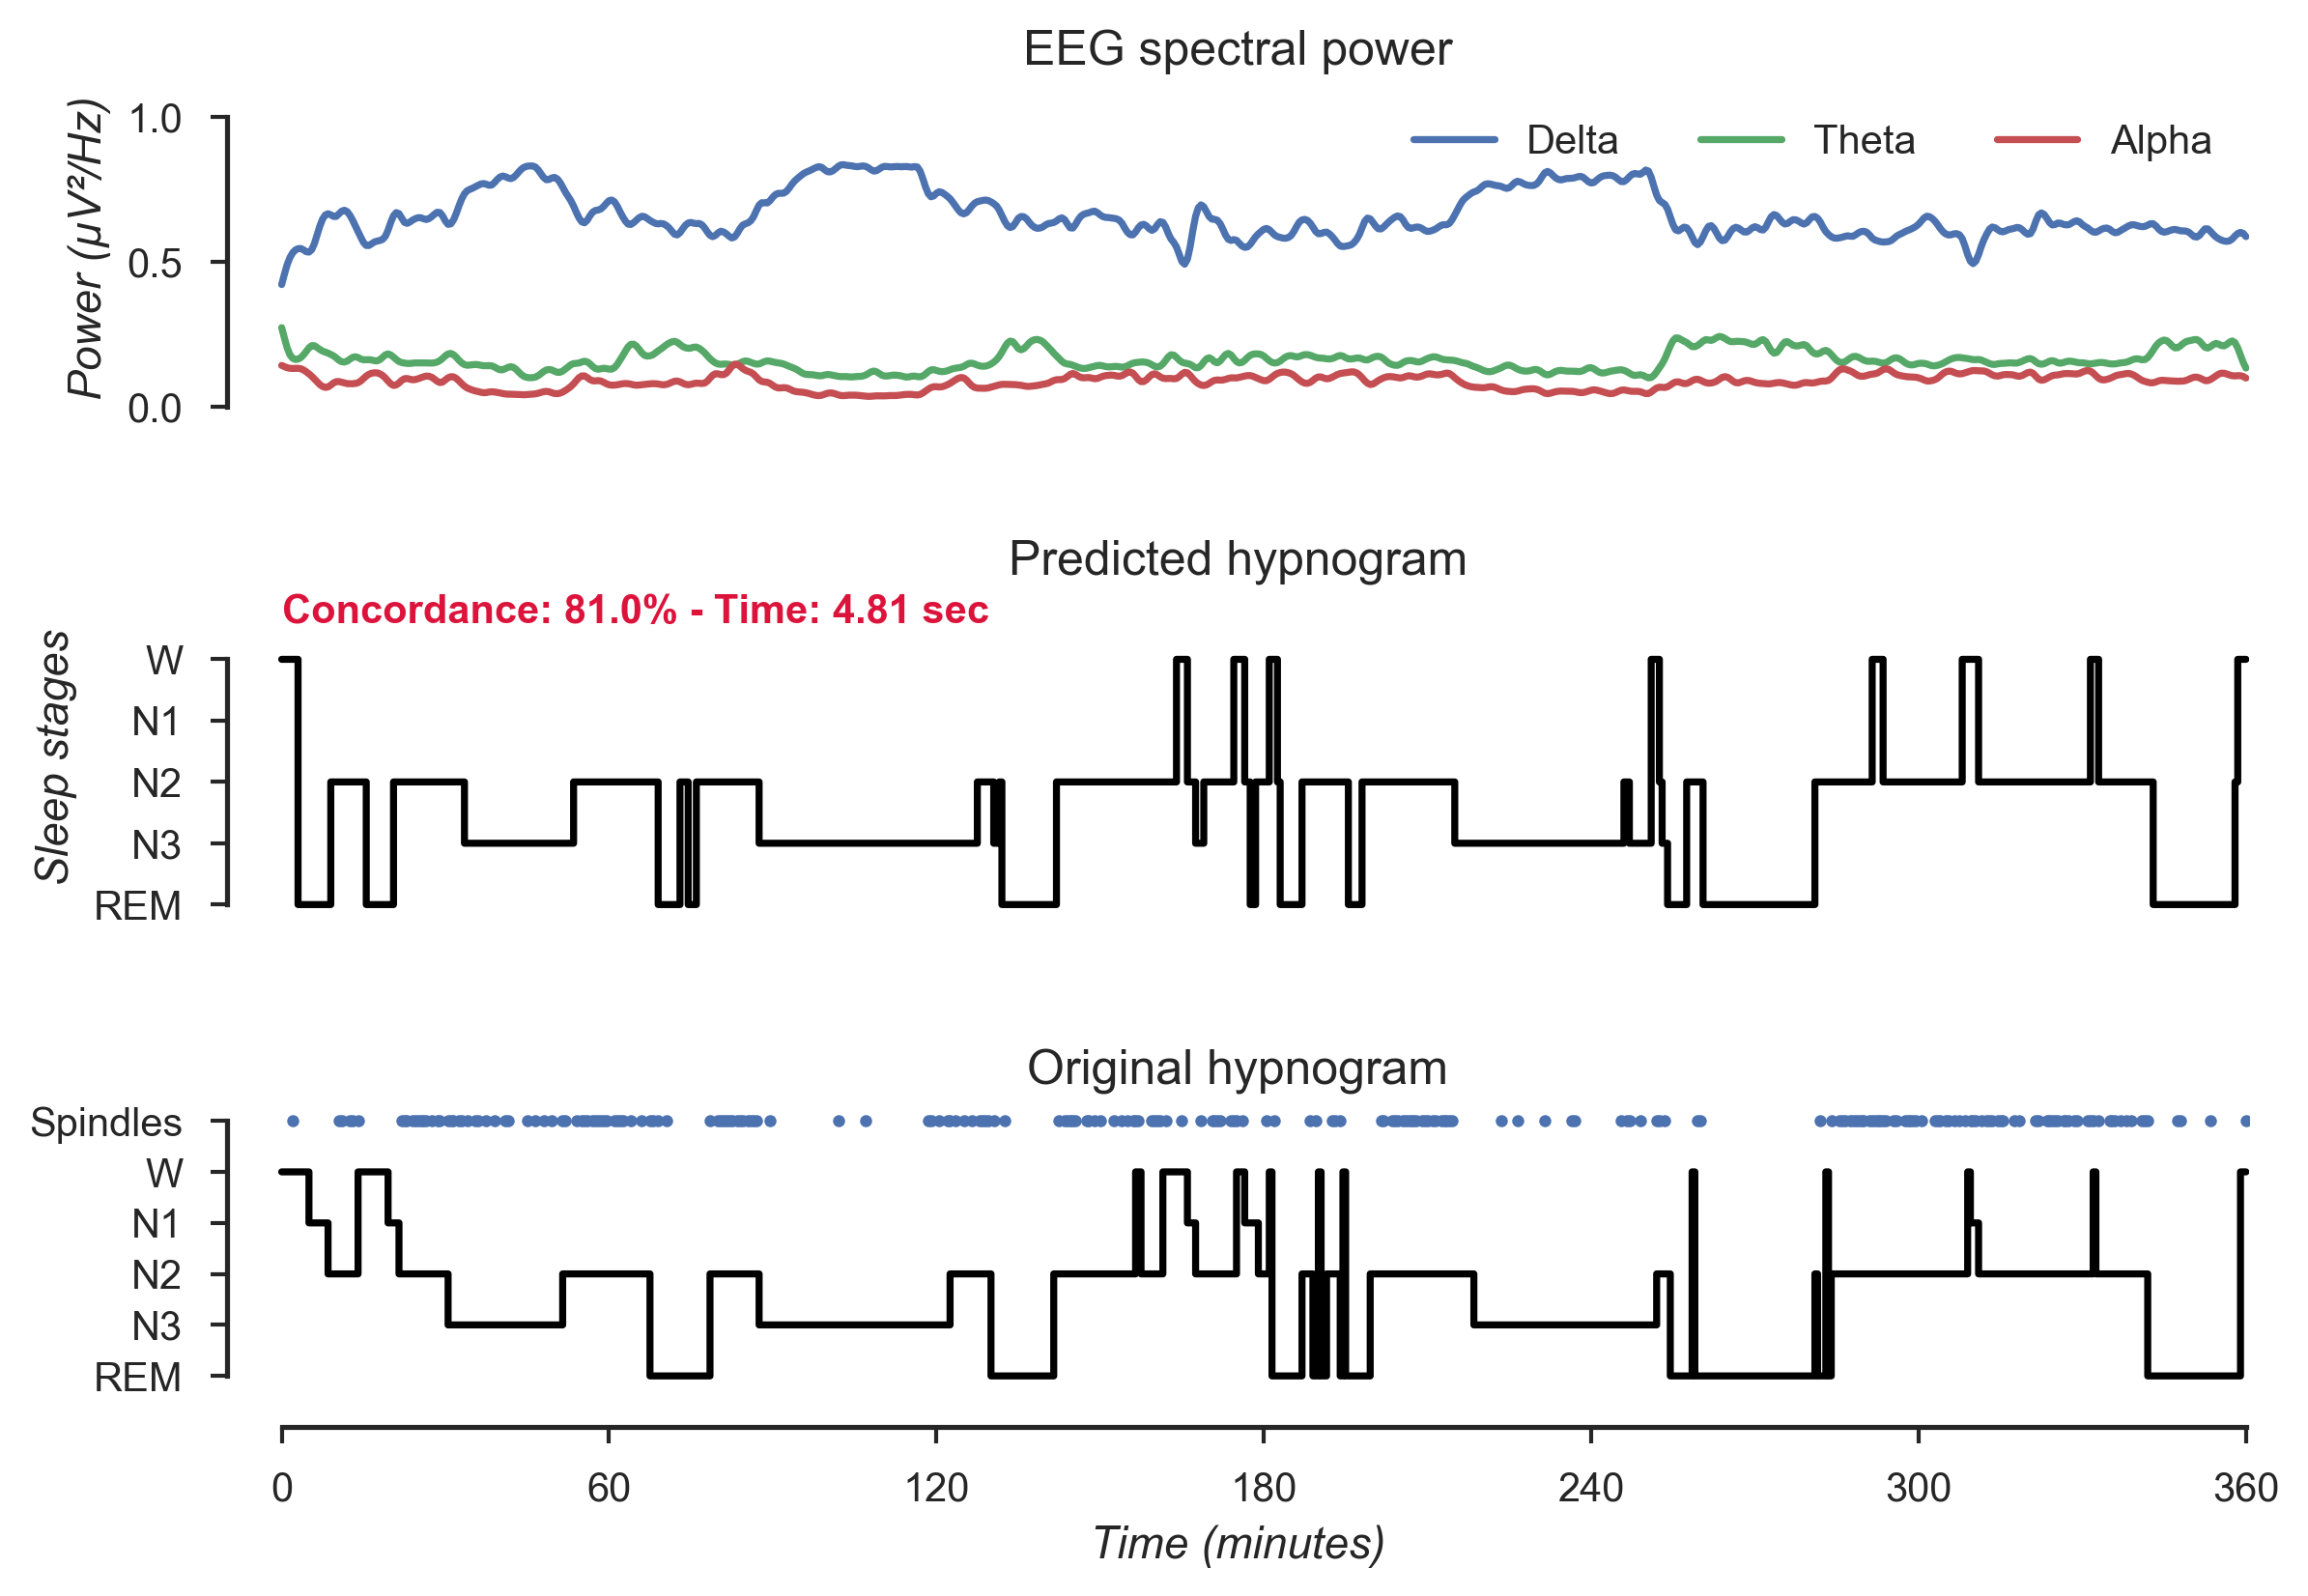
\includegraphics[width=\textwidth]{Fig/Discussion/autoscore.png}
	\caption[Preliminary results of the automatic sleep scoring algorithm]{\textbf{Preliminary results of the automatic sleep scoring algorithm.} The algorithm is based on a combination of spectral features extraction (Top) and automatic detection of microstructural features (e.g. spindles, blue dots).Preliminary tests on a full night PSG recording obtained on a healthy individual, using a single central derivation (C3), showed a percentage of concordance between the predicted and the manually scored hypnogram superior to 80\% (with a running time inferior to 5 seconds).}
	\label{fig:disc:methods:future:autoscore}
\end{figure}

Because this software represents one of the very few open-source, free and exhaustive solution for sleep reading, scoring and analysis, it should reach the broadest public (including sleep researchers, students, engineers) and lead to many great collaborations. In addition, the wide range of natively supported file formats makes it possible for numerous sleep laboratories across the world to visualize and analyze their sleep data using a single, common software. For all these reasons, the development of SLEEP represents a major step forward in sleep research, and more broadly, in open science.


%%%%%%%%%%%%%%%%%%%%%%%%%%%%%%%%%%%%%%%%%%%%%%%%%%%%%%%%%%%%%%%%%%%%%%%%%%%%%%%
\cleardoublepage
\chapter{General conclusion}
\label{disc:conclusion}
